%
\begin{isabellebody}%
\setisabellecontext{upshot}%
%
\isadelimtheory
%
\endisadelimtheory
%
\isatagtheory
%
\endisatagtheory
{\isafoldtheory}%
%
\isadelimtheory
%
\endisadelimtheory
%
\isadelimdocument
%
\endisadelimdocument
%
\isatagdocument
%
\isamarkupsection{Philosophical Contributions%
}
\isamarkuptrue%
%
\endisatagdocument
{\isafolddocument}%
%
\isadelimdocument
%
\endisadelimdocument
%
\begin{isamarkuptext}%
TESTESTESTI argue that computational ethics should be useful for and interesting to philosophers for two 
reasons. First, it could serve as the basis for AI agents with the capacity for philosophically sophisticated 
ethical reasoning. For example, my project contributes an implementation of the Formula of Universal Law
that an AI agent could use to reason about the world using the categorical imperative. Second, computational 
ethics helps philosophers think about ethics in the same way that theorem provers help 
mathematicians think about math. I am not arguing that the computer can replace human reasoning or prove things
that humans theoretically couldn't do. Instead, I argue that the computer bolsters human reasoning by forcing precision due to 
the rigid syntax of a computer program. Below, I explore 
these contributions in greater detail.%
\end{isamarkuptext}\isamarkuptrue%
%
\isadelimdocument
%
\endisadelimdocument
%
\isatagdocument
%
\isamarkupsubsection{AI Agents%
}
\isamarkuptrue%
%
\endisatagdocument
{\isafolddocument}%
%
\isadelimdocument
%
\endisadelimdocument
%
\begin{isamarkuptext}%
As artifical intelligence becomes more powerful, science-fiction predictions about ``evil AI"
and calls from regulators are intensifying the need for ``ethical AI". My project contributes a ``top down" 
approach automating a particular ethical theory. My work on automating the categorical imperative 
could serve as one component of a partially or fully artificial ethical reasoner. Specifically, my 
project could be repurposed into a ``categorical imperative library" that takes as input the logical representation of a maxim 
and determines its moral status (if it is obligatory, prohibited, or permissible).

As it stands, my project can evaluate the moral status of maxims represented in my logic and potentially 
serves as one component of an ``ethics engine" that an AI agent could use to make ethical decisions.
For example, my system could be combined with an input parser to translate moral dilemmas as represented 
to the AI agent into maxims in my logic. The ouput of my system could be fed into an output 
parser to translate this output into a prescription for the action the AI agent should take.
Figure \ref{fig:AIengine} depicts the workflow of this example ethics engine.%
\end{isamarkuptext}\isamarkuptrue%
%
\begin{figure}
\centering
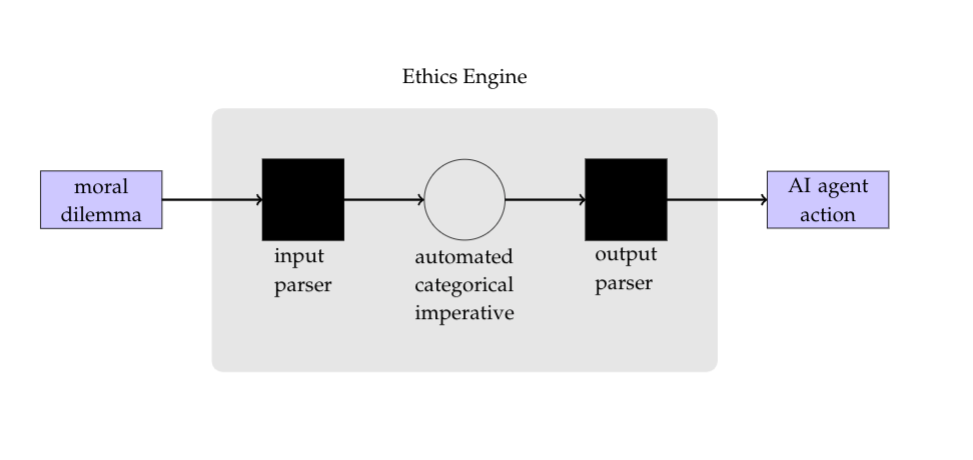
\includegraphics[scale=0.4]{AI_engine.png}
\caption{An example of an ethics engine for an artificial agent. I contribute the automated 
categorical imperative component.} \label{fig:AIengine}
\end{figure}
%
\begin{isamarkuptext}%
In this workflow, an AI agent is faced with a moral dilemma in some internal representation. This 
internal representation would need to be translated by an input parser into an appropriate logical representation, i.e. 
a circumstance, act, goal tuple. This input parser is the most technically and ethically challenging 
component of the system. It is this input parser that determines which circumstances are ``morally relevant"
for a maxim, a judgement that requires commonsense reasoning and knowledge about moral relevance. Translating 
 everyday situations into appropriate maxims is the bulk of the work that a Kantian human being does when making decisions. 
Common misconceptions about Kantian ethics\footnote{For example, some wonder why the FUL doesn't prohibit
gay sex, as the maxim ``marry someone of the same sex" appears to result in human extinction when 
universalized. The solution to this dilemma is that the maxim a gay person acts on is usually something 
of the form, ``marry the person you love because you love them," which is perfectly reasonable to 
universalize.} often result from incorrectly formulated maxims, and the entire field of 
applied Kantian ethics is devoted to generating the right kinds of maxims to test. For more discussion 
of challenges involved with defining morally relevant circumstances, see Section UNWRITTEN.

This representational
question will be one of the biggest hurdles to actually using my categorical imperative library 
in an AI ethics engine. Currently, it may be reasonable for a human being to perform the role of the input
parser. Once an AI agent stumbles onto an ethical dilemma, a human being could take over, formulate 
the right question, and feed it into the categorical imperative library to see what action the categorical 
imperative would prescribe. This may actually be a feature, not a bug. 
Proponents of the ``human-in-the-loop" model argue that fully automated decision-making is doomed 
to ethical failure, and that the inclusion of a human being injects common-sense sanity into otherwise 
dangerous decisions\footnote{For more discussion of different models of AI ethics, see Section UNWRITTEN}.  

It is likely that, regardless of the strengths of the human-in-the-loop model, fully automated AI 
agents will exist. Even if developing this kind of AI is irresponsible,
such developments are likely and will require ethics engines, or risk no consideration of ethics at all. Even if 
fully automated AI is scary, such AI with automated ethics is better than such AI without. 
In such a world, the input parser in my ethics engine would have to be automated. This would require 
that the parser translate the AI agent's internal representation to the appropriate logical representation.
The input parser would need enough common sense reasoning to determine what circumstances are morally 
relevant to a maxim. This is a question that, like all of ethics, philosophers debate robustly
\footnote{\citet{powers} identifies this as a challenge for automating Kantian ethics and briefly sketches 
solutions from \citet{constofreason}, \citet{silber}, and \citet{rawlsconstructivism}. }. 
It is likely that, just as different implementations of automated ethics choose 
a particular ethical theory and implement it, different implementations of such an input parser would 
need to adopt different interpretations of commonsense reasoning and morally relevant circumstances.
Automating this level of commonsense reasoning would represent signifiant technical progress in 
computational ethics.

Once the input has been parsed, either by a human or a machine, into  a sentence in my logic, my 
project can evaluate its moral status using my implementation of 
the FUL. Concretely, my project would return a value indicating if the maxim is obligatory, permissible, 
or prohibited. The maxim would be prohibited if it fails the universalizability test, permissible if it passes, and obligatory 
if its negation fails the universalizability test. All three of these properties amount to testing if a 
certain theorem holds or not in my logic, a calculation that I demonstrate in my tests. 

This output could then be converted into some actionable, useful response with another output parser, 
and then passed back to the AI agent. For example, if the AI agent is equipped to evaluate natural language prescriptions, the 
status of the maxim could be parsed into a natural language sentence. This output will be passed back 
to the AI agent, which will use it to make a decision. The input parser, categorical imperative library, 
and output parser together constitute an ``ethics engine" that AI agents could use as a black box 
implementation of an ethical theory. 

The ethics engine depicted above is a high-level example of one way to use my project to guide an artifical agent. The 
upshot is that an automated version of the categorical imperative could become part of the ethical engine 
for an AI agent, with much work to parse the input and the output. Effectively, the kind 
of automated ethics I implement could be a library that AI developers use to give AI agents the capacity for 
sophisticated ethical reasoning faithful to philosophical literature. This represents an improvement 
over existing ethics engines, which rarely attempt to capture the complexity 
of any ethical theory that philosophers plausibly defend. Moreover, a logic programming approach 
is potentially more explainable than a black-box deep learning approach, as theorem provers like 
Isabelle can explicitly list the axioms used to generate moral prescriptions. For more on how my project 
is situated among other work in automated ethics, see Section Related Work.%
\end{isamarkuptext}\isamarkuptrue%
%
\isadelimdocument
%
\endisadelimdocument
%
\isatagdocument
%
\isamarkupsubsection{Computational Philosophy%
}
\isamarkuptrue%
%
\endisatagdocument
{\isafolddocument}%
%
\isadelimdocument
%
\endisadelimdocument
%
\begin{isamarkuptext}%
Above I explained how my system offers a mechanism for humans to build ethical AI agents. I also 
argue that computational ethics is a mechanism for computers to help humans think differently about 
philosophy. Just as theorem provers make mathematics more efficient and push mathematicians to think 
precisely about the phenomena they are modelling, computational ethics can help philosophers think more precisely about 
philosophy. Below I share a personal example of the kind of philosophical insight that computational ethics 
can prompt and analyze the value that this tool offers to philosophers.%
\end{isamarkuptext}\isamarkuptrue%
%
\isadelimdocument
%
\endisadelimdocument
%
\isatagdocument
%
\isamarkupsubsubsection{Example of a  Philosophical Insight%
}
\isamarkuptrue%
%
\endisatagdocument
{\isafolddocument}%
%
\isadelimdocument
%
\endisadelimdocument
%
\begin{isamarkuptext}%
As I implemented a formalization of the categorical imperative using an interactive theorem prover, 
I discovered logical insights. These logical insights led to a philosophical 
insight that was novel to me and is potentially novel to the field.  While this 
insight could have been reached without the help of the computer, my system's logical results provoked
an interesting philosophical conversation. Effectively, the system spat out a logical principle, and 
I examined the philosophical plausibility of this principle for the ethical 
theory I am formalizing. In this section, I will first present the logical insight, then the 
philosophical insights, and then its implications for a debate about self-doubt. I will then
generalize my personal experience and argue that computational ethics is a new, useful methodology 
for philosophers.

I arrived at the logical insight while testing my formalization of the FUL. I realized
that my formalization was inconsistent unless I specified that the FUL only held for ``well-formed maxims,"
such that neither the act nor goal were already achieved in the given circumstances. Precisely, 
a circumstance, act, goal tuple (c, a, g) is well-formed if $(\neg (c \longrightarrow a) ) \wedge 
(\neg(c \longrightarrow g))$. This provoked the philosophical insight that maxims of this form, in which 
the act or the goal has already been accomplished in the given circumstances are ``vacuous" because 
any prescriptions they generate have already been acted on or violated. The notion of a vacuous maxim
has implications for debates about ethical self-doubt and self-confidence or self-respect.

Below, I document the process used to arrive at the logical insight that the FUL is inconsistent if it
holds for maxims in which $(c \longrightarrow a) \wedge (c \longrightarrow g)$. For those uninterested
in the details of this exploration, it suffices to understand that I used Isabelle to show that if the 
FUL holds for badly formed maxims, then it is inconsistent. After I realized that my formalization was 
inconsistent, I made many failed attempts to diagnose and fix the problem before reaizing that the problem 
lay in badly formed maxims. 

\emph{Logical Insight}

First, I used Sledgehammer to show that my formalization of the FUL\footnote{The full logical representation is \isa{FUL{\isadigit{0}}\ {\isasymequiv}\ {\isasymforall}c\ a\ g\ s{\isachardot}\ not{\isacharunderscore}universalizable\ {\isacharparenleft}c{\isacharcomma}\ a{\isacharcomma}\ g{\isacharparenright}\ s\ {\isasymlongrightarrow}\ {\isasymTurnstile}prohibited\ {\isacharparenleft}c{\isacharcomma}\ a{\isacharcomma}\ g{\isacharparenright}\ s}.}
resulted in a contradiction. Sledgehammer was able to tell me which axioms it used to complete 
this proof, showing me that my formalization contradicted the axiom O\_diamond, which states that an 
obligated term cannot contradict its context\footnote{The full form of the axiom is 
$ O \{ A \vert B \} \longrightarrow \diamond (B \wedge A)$}. 
O\_diamond formalizes the principle ``ought implies can" and requires that if A is obligated in context 
C, that A is possible in context C. I hypothesized that there was some tension between 
the antecedent of the FUL, which states that all agents act on the maxim, and the consequent, 
which states that the maxim is prohibited. If the maxim has already been acted on, then not acting on it
is impossible. Thus, the generated prohibition is impossible to obey, so the ought implies can principle
and axiom O\_diamond are violated.

I then experimented with modifications of the FUL, which I eventually abandoned. I tried universalizing the maxim 
at a world other than the current world and defining non-contradictory maxims, in which the maxim's 
circumstances do not contradict the maxim's act. I noticed that, no matter what modifications I made, 
Nitpick was timing out when looking for a model and Sledgehammer wasn't able to find a proof of
inconsistency. Isabelle's proof tools weren't able to tell me if my modifications were 
consistent or not. I suspected that something about my implementation was too slow, perhaps due to 
my liberal use of quantifiers\footnote{Benzmueller warned me that as 
I added quantifiers to the theory, Isabelle's automated proof tools may start to time out.}. 

Isabelle's model checker Nitpick performs an optimized version of a brute force model search, in which it generates many models
and checks if they satisfy the given maxims. I suspected that Nitpick 
was checking large models that exhausted its 
time limit, especially due to the logical complexity of my theory. 
To reduce the logical complexity, I decided to specify the exact number of maxims 
in the system by passing as an argument to Nitpick the cardinality of my desired model. Nitpick no longer
timed out, but it could not find a satisfying model with cardinality 1, and thus could not demonstrate
that my modified FUL was consisteny.
 This puzzled me, as I felt that I could construct a pencil-and-paper 
model with a single world and term in which my modified formalizations were consistent.

Instead of specifying the cardinality of the model, I decided to tell Nitpick exactly how many 
maxims there were in my system by defining them as constants. I defined a particular 
(circumstance, act, goal) tuple as a constant. Instead of
stating that the FUL held for all maxims, I stated that the FUL held for the specific maxim formed by this tuple.
While before I added the axiom $\forall (c, a, g) \text{\emph{FUL holds for maxim}} (c, a, g)$, I now added constants $(c, a, g)$ 
and added the axiom $\text{\emph{FUL holds for maxim}} (c, a, g)$. By specifying the circumstance, act, and goal 
as constants, I removed the external universal quantifier, thus removing a layer of logical complexity.

To my surprise, Nitpick not only returned quickly, it was able to show that the FUL was consistent!

This result was counterintuitive—after all, what is the difference between a model of cardinality 
1 and a model with one constant object? Why is quantifying over a tiny number of maxims different
 than analyzing a single maxim? Professor Amin pointed out that, as constants, the 
circumstances, act, and goal were all distinct. When they were quantified over, 
they could be identical. To formalize this idea, I defined a maxim as \isa{well{\isacharunderscore}formed\ {\isasymequiv}\ {\isasymlambda}{\isacharparenleft}c{\isacharcomma}\ a{\isacharcomma}\ g{\isacharparenright}\ s\ w{\isachardot}\ {\isasymnot}\ c\isactrlbold {\isasymrightarrow}g\ w\ {\isasymand}\ {\isasymnot}\ c\isactrlbold {\isasymrightarrow}a\ s\ w}. In propositional 
logic, a circumstance, act, goal tuple (c, a, g) is well-formed if $(\neg (c \longrightarrow a) ) \wedge 
(\neg(c \longrightarrow g))$. I tested my hypothesis by modifying my axiom to instead read $\forall$\emph{maxim
(maxim is well-formed} $\longrightarrow$ \emph{FUL holds for maxim}). This version of the FUL was indeed consistent!

To summarize, I realized that my initial attempt at formalizing the FUL was inconsistent because 
it required that the FUL hold for badly formed maxims, in which the circumstances entail the act or 
goal. The logical insight was that if FUL holds for maxims in which $(c \longrightarrow a) \vee 
(c \longrightarrow g)$, then the logic will be inconsistent.

\emph{Philosophical Insight}

SAY INCERDIBLE DIFFICULT WITHUT COMPUTER because computer looks for edge cases and makes assumptions precise.
it's an insight precisely because philosophers would never think of this edge case bc it's stupid.

Once I realized this logical property, I tried to understand its philosophical plausibility. I 
wanted to philosophically test the hypothesis that maxims in which  $(c \longrightarrow a) \vee 
(c \longrightarrow g)$ are not valid inputs to the FUL. I concluded that because vacuous maxims neither 
change an agent's behavior nor generate meaningful obligations, they are not the right kinds of questions 
for practical reasoners to be asking. They cannot be action-guiding and are thus not the kind of problem that 
ethics should be concerned with. Moreover, under the Kantian account of the will, the very act of asking 
if a vacuous maxim is prohibited generates a contradiction by undermining the will's authority over itself. 

I define a vacuous maxim as one in which the circumstances entail either the act or the goal and argue 
that such maxims can't meaningfully guide action. Consider the example vacuous maxim, ``when eating 
breakfast, I will eat breakfast in order to eat breakfast." This 
maxim isn't clearly obligatory or prohibited, but there is something empty about it. Acting on this
 maxim could never result in any actual action. If an agent adopts this maxim, 
they decide that, in the circumstances ``eating breakfast" they will perform the act ``eating breakfast"
for the purpose ``eating breakfast." In these circumstances, the act has 
already been performed! Treating this maxim a law for yourself or a principle to live by doesn't change 
how you live your life. If you adopt this maxim, when you are eating breakfast, you eat breakfast, 
but this statement is already tautologically true. 

Not only does a vacuous maxim fail to prescribe action, any obligations or prohibitions it 
generates have already been fulfilled or violated. If a vacuous 
maxim generates a prohibition, then this prohibition would be impossible to obey. 
It is impossible to not eat breakfast while eating breakfast, because the circumstances assume that the 
act has happened. On the other hand, if a vacuous maxim generates an obligation, then the obligation 
will have already been fulfilled. If you are required to eat breakfast while eating breakfast, then you've 
already fulfilled your obligation because the circumstances assume that the act has happened. Thus, 
a vacuous maxim does not actually guide action because it doesn't generate new obligations or 
prohibitions that could ever be acted on. 

Because vacuous maxims can't prescribe or alter action, they are not practically action-guiding and 
thus are not the right kinds of maxims for practical reasoners to evaluate. Moreover, insofar as ethics 
is supposed to guide action, vacuous maxims cannot be part of this project. Vacuous maxims
will have no bearing on what someone should do. Practical reason
is the kind of reason that helps us decide what we should do. 
A practical reasoner asks moral questions not as a mental puzzle or out of curiosity, but 
in order to decide how to act. Practical reason is action-guiding, but a vacuous
 maxim can never be action-guiding because it prescribes no new
actions or obligations. It is not the kind of maxim that a practical reasoner should consider, because it
will have no bearing on what the agent should do. 
There is no explicit prohibition against a vacuous maxim like the breakfast example above, but it 
is the wrong kind of question for a practical reasoner to ask. An ordinary person trying 
to navigate the world would never need to ask that kind of question. If ethics is meant 
to guide action, then badly formed maxims are not questions for ethics, because they could never guide 
action.

Above I argued that vacuous maxims are not the kind of principle that a practical reasoner should 
evaluate, and are thus not the right kind of question for ethics. Kantians can make an even stronger claim
about vacuous maxims—because maxims are laws that you give to yourself, asking if you should will 
a maxim as you will it undermines your will's law-giving ability. The circumstances of a vacuous maxim 
already assume that the agent has willed the maxim. Under the Kantian acount of willing, this act 
of willing a maxim is equivalent to giving the maxim to yourself as a law. When you will a maxim, you
adopt a law to make the maxim your end and commit yourself to be its cause. You cannot simultaneously 
commit yourself to a maxim and ask if you should be committing to it. To 
will the maxim is to adopt it as law—so the question, ``should I be 
willing this?" is paradoxical. Either you haven't actually made the maxim your law (and thus haven't yet 
committed yourself to it), or you aren't actually asking the question (because the decision has already been made).
Because a maxim is a law that you give to yourself, you cannot question it absent a sufficient reason 
(such as a change in the circumstances). To question a law arbitrarily is to not regard it as a law at all.
This kind of questioning amounts to questioning the will's authority over itself, but this is 
impossible. The will definitionally has authority over itself, for that is what it is to be a 
will. 

A skeptic may argue that we do often ask ``should I be doing this?" as we do something. What do we mean when 
we ask this question? In what sense are we trying to evalute the moral status of a vacuous maxim?
Can this kind of question ever be valid? To understand this worry, I consider the maxim, 
``When dancing, I should just dance for the sake of dancing."\footnote{Maybe cite Korgsaard since the
dancing thing is her example.} While this maxim appears to be vacuous (the 
circumstance `dancing' implies the act and goal of dancing), it's a question that practical reasoners 
do ask. I argue that there are this maxim is actually misunderstood and, when interpreted correctly,
it no longer poses as a counterexample to my complaints about vacuous maxims.

Under one reading of this maxim, "I should just dance" is actually referring to a different act than the circumstance ``when dancing". 
The circumstance ``when dancing" refers 
to rythmically moving your body to music, but ``I should just dance" refers to dancing without anxiety, 
completely focused on the joy of dancing itself. More precisely, this maxim should read ``When 
dancing, I should abandon my anxiety and focus on dancing for the sake of dancing." This maxim when so 
modified is not vacuous at all—abandoning anxiety and focusing on dancing is an entirely different act 
from moving your body rythmically to music. This maxim is actually well-formed, and thus doesn't
pose a problem for my argument. It is entirely plausible to tell yourself ``When I am dancing, I should focus 
on dancing for the sake of dancing itself." The circumstances do not entail the act or the goal because 
they refer to different meanings of the word dancing. Any valid reading of this maxim will have the structure above, 
in which the act is actually different from the circumstances. A reasoner cannot accept their will 
as law-giving or commit themselves to an act and simultaneously question the act. Either they must be 
questioning a different act or they must have recieved new information to prompt the questioning, 
modifying the circumstances of the original maxim. 

Another related worry has to with maxims that we do in fact think are prohibited. Consider the maxim modified to 
read ``When dancing and seeing a child drowning, I should dance for the sake of dancing." Clearly this 
maxim is fit for moral evaluation, and we expect a moral theory to prohibit this maxim. The circumstances 
``When dancing and seeing a child drowning" appear to entail the act of dancing, and the maxim thus 
appears vacuous. Once again, this maxim is formulated incorrectly. In this case, the question 
that the agent is actually asking themselves is ``should I continue dancing?" That is the 
maxim that they will adopt or reject. They mean to ask if they should stop dancing and go help the child. 
Dancing at the current moment and dancing at the next moment are different acts, and the circumstances 
imply the former but not the latter. A vacuous maxim would have circumstances and act both 
``dancing at moment t," but this maxim has circumstances ``dancing at moment t" and act ``dancing 
at moment t+1." This is a kind of temporal error that has bearings for other debates in ethics as well. 
Specifically, the confusion between circumstances and acts that occur at different times (as in this example) and circumstances 
and acts that occur at the exact same time has bearing on self-doubt, as I will argue next.

\emph{Implications for Self Doubt and Self Respect}

The dancing maxim can also be understood through the lens of self-doubt. Under this 
reading, the question ``When I am dancing, 
should I be dancing for the sake of dancing?" is the agent asking, ``Am I doing the right thing 
right now?" Unlike the drowning example, the agent is not asking about the next moment, but is expressing doubt about the 
moral validity of their behavior at this current moment. I do not want to argue that self-doubt always
 undermines the will—after all, self-doubt plays an important role in moral 
reasoning and is often the mark of a thoughtful agent. I argue instead that questions of self-doubt
do not actually involve vacuous maxims, for these are not the maxims that the agent is doubting. Indeed,
this example demonstrates that the tension between self-doubt and self-respect arises from a 
mistaken characterization of questions of self-doubt as questions about vacuous maxims.
I first explain the tension between self-doubt and self-respect in epistemology, then 
explain the parallel tension in ethics, and finally present a resolution of this tension.

In epistemology, there is a tension between the rational requirement to believe in yourself and the 
value of self-doubt, in moderation. Christensen presents the ``principle of self-respect," which requires 
that any rational agent refrain from believing that they have mistaken beliefs \cite[4]{christensen}. For example, I cannot 
rationally both believe that the sky is blue and believe that I believe that the sky is green. In other words, I cannot 
disapprove of my own credences. Christensen argues that this principle, which he abbreviates to SR, holds because 
a perfectly rational agent can make accurate and confident judgements about what they believe. If this 
is the case, violating SR results in a simple contradiction \cite[8-9]{christensen}. 

While most philosophers accept some version of SR\footnote{Van Fraassen, Vickers, Koons \cite[5]{christensen}}, 
Roush argues that the principle must be modified in order to account for healthy epistemic 
self-doubt. She argues that, while pathological second-guessing is roundly criticized, we are generally 
imperfect beings, and some sensitivity to our own limitations is a virtue \cite[2]{roushselfhelp}. Indeed, even Christensen 
acknowledges that total self-confidence is an epistemic flaw \cite[1]{christensen}. Thus, there is tension between the rational
requirement to respect our authority as believers and the practical reality that we are often wrong. 

This debate between self-respect and self-doubt in epistemology also applies to ethics. When we 
decide to act and commit ourselves to acting, we cannot simultaneously doubt the 
validity of our action. If human behavior is purposive, then the very act of committing oneself implies 
that one has sufficient reasons for committing oneself. These reasons may be flawed, but in making the 
commitment, the reasoner has accepted them. It is contradictory to claim that someone commits and questions 
simultaneously, because commitment itself implies a resolution to the question. Either the commitment 
is not real, or the question is not. I will call the principle that 
one cannot will a maxim and simultaneously question if they should will that maxim
``ethical self-respect" or ESR.

On the other hand, self-doubt is an important part of ethical reasoning. Just as believers are often 
mistaken, so are practical reasoners. An agent with perfect confidence, who is always sure that they 
are doing the right thing, is clearly not thinking deeply enough about their obligations. Some degree
of ethical self-doubt is normal and likely desirable. Thus, there is a tension between the rational
requirement of ESR and the intuitive validity of ethical self-doubt (ESD).

To resolve this tension, I return to my earlier example of a dancer. Imagine Sara is dancing at a 
weddding, when, in a moment of angst, she asks herself, ``Should I really be dancing right now?" 
What question is she asking here? The immediate answer is that she asking if the maxim, ``When dancing 
at your friend's wedding, dance for the sake of dancing" is a permissible maxim to act on. Notice that t
he maxim in question is vacuous: the circumstance ``when dancing at a friend's wedding" implies the act 
``dance." Because this is a vacuous maxim, it cannot be the maxim that she is questioning, for adopting 
this maxim could not have changed her behavior at all. Sara is asking a question about her actions and 
their validity. Any conclusions about the validity of a vacuous maxim would not help her, first because 
the maxim has no effect on her action, and second because any such validity would be a foregone conclusion
as she has already adopted the maxim. As 
I argued above, no practical reasoner can coherently ask themselves whether a vacuous maxim is 
valid or not without undermining their will, which is a contradiction. Thus, under 
the interpretation of self-doubt as a vacuous maxim, the tension between ESR and ethical self-doubt 
appears irresolvable. Those committed to this interpretation must abandon one principle or the other.

To resolve this issue, I turn to another interpretation of ethical self-doubt. Under this interpretation, 
when Sara asks, ``Should I really be dancing right now?" she wants to know if the maxim that 
resulted in the current moment when she is on the dance floor was actually 
the right thing to will. She is asking if she made the right 
decision in the past, when she decided to dance. The maxim that initiated the dancing would be something 
like ``When at a wedding, dance for the sake of dancing." This is the maxim that she is currently acting 
on, not the vacuous maxim ``When dancing, dance for the sake of dancing." Under this interpretation, 
there is no tension at all between self-doubt and self-respect. It is perfectly valid for a reasoner 
to doubt their prior moral judgements, just as it is perfectly rational for a believer to doubt their 
past beliefs \cite[3-4]{christensen}. Such doubt does not undermine the reasoner's decision-making 
capacity and is thus perfectly consistent with ethical self-respect. 

Not only does this second interpretation resolve the tension between ESR and ESD, it also more accurately 
tracks the operation of practical reason. As argued above, a practical reasoner would never ask themselves 
whether or not to will a vacuous maxim, because such a maxim would generate no meaningful obligations. 
Adopting such a maxim would not alter their behavior in any way. Moreover, the fact that a practical 
reasoner never adopts a vacuous maxim demonstrates the cause of the tension between ESR and ESD.
The tension itself arises from a misreading of questions of self-doubt as questions about 
the evaluation of vacuous maxims. A question of self-doubt cannot refer to a vacuous maxim and must 
instead refer to a well-formed maxim about the agent's past decision-making. As seen before, cases where 
agents appear to ask themselves about vacuous maxims are mistaken about the maxim in question, because 
such a question could never yield a useful answer for a practical reasoner.%
\end{isamarkuptext}\isamarkuptrue%
%
\isadelimdocument
%
\endisadelimdocument
%
\isatagdocument
%
\isamarkupsubsubsection{The Value of Computational Ethics%
}
\isamarkuptrue%
%
\endisatagdocument
{\isafolddocument}%
%
\isadelimdocument
%
\endisadelimdocument
%
\begin{isamarkuptext}%
I will now generalize from the personal insight reached above to the methodological value of 
computational ethics for philosophers.
I do not argue that computational ethics, as it stands today, uncovers philosophical insights that humans have not reached
or are incapable of reaching. After all, my understanding of a well-formed maxim could 
very well exist in the literature and certainly could be reached by a philosopher without any 
computational tools. Instead, I argue that computational tools prompt philosophers to ask questions that 
lead to insights. Philosophers already value precision, and the computer forces precision and makes formal
reasoning easier. Computational 
ethics can serve as another tool in a philosopher's arsenal, like a thought experiment or counterexample.
While the technology is not yet mature enough and easy enough to use to become widespread in philosophy
departments, technical progress could turn computational ethics into an easy-to-use tool for philosophers
that doesn't require any specialized progamming or logical knowledge.

The first contribution of computational ethics is precision \footnote{TODO: this article discusses 
benefits of precision: bookmarked}. Much of analytic philosophy involves 
making a particular concept precise. Thought experiments, arguments, counterexamples, and examples 
illustrate features of a concept in the hope of making the concept itself more precise. Computational 
ethics can help philosophers reach this goal of precision in another, potentially easier, way. 
Representing a philosophical idea in logic and implementing it in an interactive theorem prover requires 
making the idea precise to a degree that ordinary discussion can result in, but does not necessarily require. The initial representation 
of an idea in a logic requires making its form precise. For example, 
as I formalized the notion of a maxim, I had to understand its components and define it as a 
circumstance, act, goal tuple. Moreover, Isabelle's strict typing system required that I define 
coherent, consistent types for each of these entities and for a maxim as a whole. This requires understanding 
what role each of these components play in the FUL and assigning them each a type. In my example, I 
concluded that circumstances and goals are terms, which can be true or false at a world, and acts are 
open sentences, which are true for a particular subject at a particular world. This precision is possible 
without computational tools, but computational ethics forces a level of precision that ordinary discussion 
does not demand. Type fuzziness and overloaded definitions are all too common in philosophical writing and 
discussion (would be cool to cite some famous debate revolving around this idea), but computers don't 
allow this kind of imprecision.

Another, related benefit of computational ethics is that it makes formal ethics far less tedious. 
Certain subfields, such as philosophy of language, see such benefit in precision that they already 
use symbolic logic to represent philosophical concepts, just as mathematicians use symbolic logic to 
represent mathematical concepts. Some of this work requres tedious pencil and paper proofs to prove 
theorems, even when many of these theorems may not generate relevant philosophical insights. Interactive 
theorem provers make formal logic more accessible. Isabelle can complete a proof, starting from first principles, 
in a matter of seconds that would take a logician pages to complete. Similarly, Nitpick can generate 
examples or counterexamples to a proposition in a brute force manner. The computer can generate hypotheses
that philosophers can then think about, just as it did for me to prompt the insight above.

Just as calculators make arithmetic more accessible, computational ethics does the same for formal philosophy. 
Not all philosophy can or will 
be formalized or automated—after all, calculators didn't make accountants or mathematicians obsolete. Just as computers 
reduce the tedium in other aspects of our life, they can reduce the tedium involved in formal logic to 
allow mathematicians and philosophers to focus their attention on understanding.%
\end{isamarkuptext}\isamarkuptrue%
%
\isadelimdocument
%
\endisadelimdocument
%
\isatagdocument
%
\isamarkupsubsubsection{Looking Forward%
}
\isamarkuptrue%
%
\endisatagdocument
{\isafolddocument}%
%
\isadelimdocument
%
\endisadelimdocument
%
\begin{isamarkuptext}%
Computational ethics is at its infancy. The use of theorem provers in mathematics is just now beginning 
to make headway \cite{buzzardvideo}, even though theorem provers were first invented in the 1960's \cite{historyofITP}. In contrast, the first attempts to use theorem 
provers for ethics occurred in the last decade. The fact that this nascent technology is already 
helping humans reach non-trivial philosophical conclusions is reason to, at the very least, entertain 
the possibility of a future where computational ethics becomes as normal for philosophers.

To the skeptic, the ethical insights uncovered by the computer are not necessarily impressive 
philosophy. Indeed, the fact that a theorem prover requires specialized knowledge outside of the field 
of philosophy indicates that the technology is nowhere near ready for universal use in philosophy 
departments. However, history indicates that as computing power increases and computer scientists make 
progress, computational ethics will become more usable. Theorem provers in mathematics began as toys 
incapable of proving that the real number 2 is not equal to the real number 1, but Buzzard showed that 
moving from such a primitive system to a tool for Fields medal winning mathematics is possible in a 
matter of years \cite{buzzardvideo}. Countless examples from the history of computer science, from the Turing 
Test to AI game playing to protein folding, demonstrate that progress in computer science can make seemingly 
obscure computer programs useful and usable in ways that exceed our wildest imaginations. Indeed, 
programmable computers themselves initially began as unwieldy punch card readers, but their current ubiquity 
need not be stated. If computer scientists and philosophers invest in computational ethics, it can 
become as much a tool for philosophy as a calculator is for for arithmetic.\footnote{Is this too like, 
lalalala fantasy of computational philosophy? Would it be less so if I did more work explaining 
the history of theorem proving for math? Is this even that important for my project?}%
\end{isamarkuptext}\isamarkuptrue%
%
\isadelimtheory
%
\endisadelimtheory
%
\isatagtheory
%
\endisatagtheory
{\isafoldtheory}%
%
\isadelimtheory
%
\endisadelimtheory
%
\end{isabellebody}%
\endinput
%:%file=~/Desktop/cs91r/paper/upshot.thy%:%
%:%24=6%:%
%:%36=8%:%
%:%37=9%:%
%:%38=10%:%
%:%39=11%:%
%:%40=12%:%
%:%41=13%:%
%:%42=14%:%
%:%43=15%:%
%:%44=16%:%
%:%53=18%:%
%:%65=20%:%
%:%66=21%:%
%:%67=22%:%
%:%68=23%:%
%:%69=24%:%
%:%70=25%:%
%:%71=26%:%
%:%72=27%:%
%:%73=28%:%
%:%74=29%:%
%:%75=30%:%
%:%76=31%:%
%:%77=32%:%
%:%80=36%:%
%:%81=37%:%
%:%82=38%:%
%:%83=39%:%
%:%84=40%:%
%:%85=41%:%
%:%88=43%:%
%:%89=44%:%
%:%90=45%:%
%:%91=46%:%
%:%92=47%:%
%:%93=48%:%
%:%94=49%:%
%:%95=50%:%
%:%96=51%:%
%:%97=52%:%
%:%98=53%:%
%:%99=54%:%
%:%100=55%:%
%:%101=56%:%
%:%102=57%:%
%:%103=58%:%
%:%104=59%:%
%:%105=60%:%
%:%106=61%:%
%:%107=62%:%
%:%108=63%:%
%:%109=64%:%
%:%110=65%:%
%:%111=66%:%
%:%112=67%:%
%:%113=68%:%
%:%114=69%:%
%:%115=70%:%
%:%116=71%:%
%:%117=72%:%
%:%118=73%:%
%:%119=74%:%
%:%120=75%:%
%:%121=76%:%
%:%122=77%:%
%:%123=78%:%
%:%124=79%:%
%:%125=80%:%
%:%126=81%:%
%:%127=82%:%
%:%128=83%:%
%:%129=84%:%
%:%130=85%:%
%:%131=86%:%
%:%132=87%:%
%:%133=88%:%
%:%134=89%:%
%:%135=90%:%
%:%136=91%:%
%:%137=92%:%
%:%138=93%:%
%:%139=94%:%
%:%140=95%:%
%:%141=96%:%
%:%142=97%:%
%:%143=98%:%
%:%144=99%:%
%:%145=100%:%
%:%146=101%:%
%:%147=102%:%
%:%148=103%:%
%:%149=104%:%
%:%150=105%:%
%:%151=106%:%
%:%160=108%:%
%:%172=110%:%
%:%173=111%:%
%:%174=112%:%
%:%175=113%:%
%:%176=114%:%
%:%177=115%:%
%:%186=117%:%
%:%198=119%:%
%:%199=120%:%
%:%200=121%:%
%:%201=122%:%
%:%202=123%:%
%:%203=124%:%
%:%204=125%:%
%:%205=126%:%
%:%206=127%:%
%:%207=128%:%
%:%208=129%:%
%:%209=130%:%
%:%210=131%:%
%:%211=132%:%
%:%212=133%:%
%:%213=134%:%
%:%214=135%:%
%:%215=136%:%
%:%216=137%:%
%:%217=138%:%
%:%218=139%:%
%:%219=140%:%
%:%220=141%:%
%:%221=142%:%
%:%222=143%:%
%:%223=144%:%
%:%224=145%:%
%:%225=146%:%
%:%226=147%:%
%:%227=148%:%
%:%228=149%:%
%:%229=150%:%
%:%230=151%:%
%:%231=152%:%
%:%232=153%:%
%:%233=154%:%
%:%234=155%:%
%:%235=156%:%
%:%236=157%:%
%:%237=158%:%
%:%238=159%:%
%:%239=160%:%
%:%240=161%:%
%:%241=162%:%
%:%242=163%:%
%:%243=164%:%
%:%244=165%:%
%:%245=166%:%
%:%246=167%:%
%:%247=168%:%
%:%248=169%:%
%:%249=170%:%
%:%250=171%:%
%:%251=172%:%
%:%252=173%:%
%:%253=174%:%
%:%254=175%:%
%:%255=176%:%
%:%256=177%:%
%:%257=178%:%
%:%258=179%:%
%:%259=180%:%
%:%260=181%:%
%:%261=182%:%
%:%262=183%:%
%:%263=184%:%
%:%264=185%:%
%:%265=186%:%
%:%266=187%:%
%:%267=188%:%
%:%268=189%:%
%:%269=190%:%
%:%270=191%:%
%:%271=192%:%
%:%272=193%:%
%:%273=194%:%
%:%274=195%:%
%:%275=196%:%
%:%276=197%:%
%:%277=198%:%
%:%278=199%:%
%:%279=200%:%
%:%280=201%:%
%:%281=202%:%
%:%282=203%:%
%:%283=204%:%
%:%284=205%:%
%:%285=206%:%
%:%286=207%:%
%:%287=208%:%
%:%288=209%:%
%:%289=210%:%
%:%290=211%:%
%:%291=212%:%
%:%292=213%:%
%:%293=214%:%
%:%294=215%:%
%:%295=216%:%
%:%296=217%:%
%:%297=218%:%
%:%298=219%:%
%:%299=220%:%
%:%300=221%:%
%:%301=222%:%
%:%302=223%:%
%:%303=224%:%
%:%304=225%:%
%:%305=226%:%
%:%306=227%:%
%:%307=228%:%
%:%308=229%:%
%:%309=230%:%
%:%310=231%:%
%:%311=232%:%
%:%312=233%:%
%:%313=234%:%
%:%314=235%:%
%:%315=236%:%
%:%316=237%:%
%:%317=238%:%
%:%318=239%:%
%:%319=240%:%
%:%320=241%:%
%:%321=242%:%
%:%322=243%:%
%:%323=244%:%
%:%324=245%:%
%:%325=246%:%
%:%326=247%:%
%:%327=248%:%
%:%328=249%:%
%:%329=250%:%
%:%330=251%:%
%:%331=252%:%
%:%332=253%:%
%:%333=254%:%
%:%334=255%:%
%:%335=256%:%
%:%336=257%:%
%:%337=258%:%
%:%338=259%:%
%:%339=260%:%
%:%340=261%:%
%:%341=262%:%
%:%342=263%:%
%:%343=264%:%
%:%344=265%:%
%:%345=266%:%
%:%346=267%:%
%:%347=268%:%
%:%348=269%:%
%:%349=270%:%
%:%350=271%:%
%:%351=272%:%
%:%352=273%:%
%:%353=274%:%
%:%354=275%:%
%:%355=276%:%
%:%356=277%:%
%:%357=278%:%
%:%358=279%:%
%:%359=280%:%
%:%360=281%:%
%:%361=282%:%
%:%362=283%:%
%:%363=284%:%
%:%364=285%:%
%:%365=286%:%
%:%366=287%:%
%:%367=288%:%
%:%368=289%:%
%:%369=290%:%
%:%370=291%:%
%:%371=292%:%
%:%372=293%:%
%:%373=294%:%
%:%374=295%:%
%:%375=296%:%
%:%376=297%:%
%:%377=298%:%
%:%378=299%:%
%:%379=300%:%
%:%380=301%:%
%:%381=302%:%
%:%382=303%:%
%:%383=304%:%
%:%384=305%:%
%:%385=306%:%
%:%386=307%:%
%:%387=308%:%
%:%388=309%:%
%:%389=310%:%
%:%390=311%:%
%:%391=312%:%
%:%392=313%:%
%:%393=314%:%
%:%394=315%:%
%:%395=316%:%
%:%396=317%:%
%:%397=318%:%
%:%398=319%:%
%:%399=320%:%
%:%400=321%:%
%:%401=322%:%
%:%402=323%:%
%:%403=324%:%
%:%404=325%:%
%:%405=326%:%
%:%406=327%:%
%:%407=328%:%
%:%408=329%:%
%:%409=330%:%
%:%410=331%:%
%:%411=332%:%
%:%412=333%:%
%:%413=334%:%
%:%414=335%:%
%:%415=336%:%
%:%416=337%:%
%:%417=338%:%
%:%418=339%:%
%:%419=340%:%
%:%420=341%:%
%:%421=342%:%
%:%422=343%:%
%:%423=344%:%
%:%424=345%:%
%:%425=346%:%
%:%426=347%:%
%:%427=348%:%
%:%428=349%:%
%:%429=350%:%
%:%430=351%:%
%:%431=352%:%
%:%432=353%:%
%:%433=354%:%
%:%434=355%:%
%:%435=356%:%
%:%436=357%:%
%:%437=358%:%
%:%438=359%:%
%:%439=360%:%
%:%440=361%:%
%:%441=362%:%
%:%442=363%:%
%:%443=364%:%
%:%444=365%:%
%:%445=366%:%
%:%446=367%:%
%:%447=368%:%
%:%448=369%:%
%:%449=370%:%
%:%450=371%:%
%:%451=372%:%
%:%452=373%:%
%:%453=374%:%
%:%454=375%:%
%:%455=376%:%
%:%456=377%:%
%:%457=378%:%
%:%458=379%:%
%:%459=380%:%
%:%460=381%:%
%:%461=382%:%
%:%462=383%:%
%:%463=384%:%
%:%464=385%:%
%:%465=386%:%
%:%466=387%:%
%:%467=388%:%
%:%468=389%:%
%:%469=390%:%
%:%470=391%:%
%:%479=395%:%
%:%491=397%:%
%:%492=398%:%
%:%493=399%:%
%:%494=400%:%
%:%495=401%:%
%:%496=402%:%
%:%497=403%:%
%:%498=404%:%
%:%499=405%:%
%:%500=406%:%
%:%501=407%:%
%:%502=408%:%
%:%503=409%:%
%:%504=410%:%
%:%505=411%:%
%:%506=412%:%
%:%507=413%:%
%:%508=414%:%
%:%509=415%:%
%:%510=416%:%
%:%511=417%:%
%:%512=418%:%
%:%513=419%:%
%:%514=420%:%
%:%515=421%:%
%:%516=422%:%
%:%517=423%:%
%:%518=424%:%
%:%519=425%:%
%:%520=426%:%
%:%521=427%:%
%:%522=428%:%
%:%523=429%:%
%:%524=430%:%
%:%525=431%:%
%:%526=432%:%
%:%527=433%:%
%:%528=434%:%
%:%529=435%:%
%:%530=436%:%
%:%531=437%:%
%:%532=438%:%
%:%533=439%:%
%:%534=440%:%
%:%535=441%:%
%:%536=442%:%
%:%537=443%:%
%:%546=446%:%
%:%558=449%:%
%:%559=450%:%
%:%560=451%:%
%:%561=452%:%
%:%562=453%:%
%:%563=454%:%
%:%564=455%:%
%:%565=456%:%
%:%566=457%:%
%:%567=458%:%
%:%568=459%:%
%:%569=460%:%
%:%570=461%:%
%:%571=462%:%
%:%572=463%:%
%:%573=464%:%
%:%574=465%:%
%:%575=466%:%
%:%576=467%:%
%:%577=468%:%
%:%578=469%:%